\subsection*{Writing, Process}
Describe the process shown on figure~\ref{fig:ielts_writing_uml_activity}.

\begin{figure}[H]
  \centering
    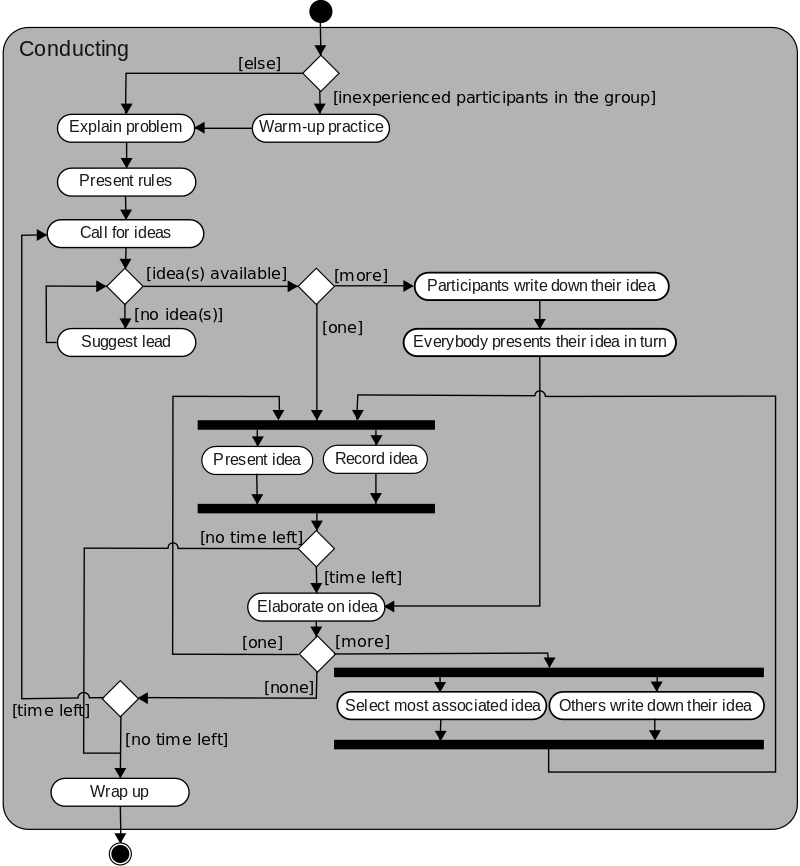
\includegraphics[width=\textwidth]{ielts_writing_uml_activity}
  \caption{Activity diagram for a guided brainstorming process.}
  \label{fig:ielts_writing_uml_activity}
\end{figure}

\begin{answer}
If there are inexperienced participants in the group a quick warm-up is performed.

Then the problem (the topic of the brainstorm) and the rules are presented and explained by a facilitator.
Rules usually contain encouragement of deferring judgement, going for quantity and providing wild and unexpected answers.

Withholding criticism is necessary to release the preasure of generating <<stupid>> ideas.

Then the participants are called for ideas. 

Each person that has an idea presents one in turn. 
The idea receives no criticism or discussion from the participants.
The group tries to combine and improve the idea and selects a few ideas to represent later.

This continues until the time is up.

Once all the ideas are captured, the group can prioritize and/or take action.
\end{answer}
